%
% teil3.tex -- Beispiel-File für Teil 3
%
% (c) 2020 Prof Dr Andreas Müller, Hochschule Rapperswil
%
\section{Der Munkres-Algorithmus (Ungarische Methode)
\label{munkres:section:teil3}}
\rhead{Der Munkres-Algorithmus (Ungarische Methode)}

Mit der ungarischen Methode können also Optimierungsprobleme gelöst
werden, die bei gewichteten Zuordnungen in bipartiten Graphen entstehen.
Mit ihr kann die eindeutige Zuordnung von Objekten aus zwei Gruppen so
optimiert werden, dass die Gesamtkosten minimiert werden bzw.~der
Gesamtgewinn maximiert werden kann. 

\subsection{Geschichte
\label{munkres:subsection:malorum}}
Die Ungarische Methode wurde 1955 von Harold Kuhn entwickelt und veröffentlicht.
Der Name ``Ungarische Methode'' ergab sich, weil der Algorithmus
weitestgehend auf den früheren Arbeiten zweier ungarischer Mathematiker
basierte: Dénes Kőnig und Jenő Egerváry.
James Munkres überprüfte den Algorithmus im Jahr 1957 und stellte fest,
dass der Algorithmus (stark) polynomiell ist.
Seitdem ist der Algorithmus auch als Kuhn-Munkres oder
Munkres-Zuordnungsalgorithmus bekannt.
Die Zeitkomplexität des ursprünglichen Algorithmus war $O(n^4)$,
später wurde zudem festgestellt, dass er modifiziert werden kann,
um eine  $O(n^3)$-Laufzeit zu erreichen.

\subsection{Besondere Leistung der Ungarischen Methode
\label{munkres:subsection:malorum}}
Die Ungarische Methode ist ein kombinatorischer Optimierungsalgorithmus, der das Zuordnungsproblem
in polynomieller Zeit löst.
Der Begriff polynomielle Laufzeit bedeutet, dass die Laufzeit des Programms
wie $n^2$, $n^3$, $n^4$, etc.~wächst und vernünftig skaliert. $n$ ist hierbei die "Grösse" des Problems.

\subsection{Unterschiedliche Anzahl von Quellen und Zielen
\label{munkres:subsection:malorum}}
Es gibt Fälle, in welchen das Ausgangsproblem keine quadratische Form besitzt. Das ist z.B dann der Fall, wenn eine 3 Mitarbeiter 4 Eignungstests abdsolvieren müssen. In diesem Fall wird in der Ungarischen Methode die Matrix künstlich mittels einer Dummy Position quadratisch ergänzt. Dummy-Positionen werden dann mit der größten vorhandenen Zahl aus der Matrix besetzt. Beispielsweise eine $4\times 3$ wird zu einer $4\times 4$ Matrix.

\subsection{Beispiel eines händischen Verfahrens
\label{munkres:subsection:malorum}}

Die ungarische Methode kann in einem einfachen händischen Beispiel
erläutert werden. Es gibt eine Ausgangsmatrix. Diese Matrix wird in mehreren Schritten immer
weiter reduziert. Anschließend erfolgen mehrere Zuordnungen. Hierbei ist zu beachten, dass
jede Zeile und jede Spalte immer genau eine eindeutige Zuordnung ergibt.
Die optimale Lösung ist erreicht, wenn genau $n$ Zuordnungen gefunden
sind.

\begin{enumerate}
\item Pro Zeile eruiert man die kleinste Zahl. Diese kleinste Zahl wird bei
allen anderen Ziffern in der jeweiligen Zeile subtrahiert.

\item Danach zieht man wiederum die kleinste Zahl in jeder Spalte von allen
Zahlen in der Spalte ab.

\item Es sollen möglichst viele Nullen markiert werden, welche freistehend sind.
(Freistehend bedeutet, sowohl in der jeweiligen Zeile und Spalte nur
eine markierte Null zu haben)

\item Jeweilige Zeilen eruieren, bei welchen keine markierte Null vorhanden sind und kennzeichnen.

\item In der vorherigen Zeile die 0 eruieren und die Spalte ebenfalls
kennzeichnen (*2)

\item Im der selben Spalte die Markierte Null eruieren und die dazugehörige
Zeile kennzeichnen (*3)

\item Alle Zeilen durchstreichen, welche KEINE Kennzeichnungen (*) haben

\item Alle Spalten durchstreichen, welche EINE Kennzeichnung besitzt! (hier, *2)

\item Kleinste Ziffer auswählen, welche nicht schon durchgestrichen sind.
(Im Beispiel ist es die Zahl 1. (Egal welche 1)

\item Die eruierte kleinste Ziffer, wird von den nicht durchgestrichenen Ziffern
subtrahiert. Danach muss die Matrix wieder komplettiert werden. (inkl. Unterstreichen)

\item Jeweilige Zahlen eruieren, welche vorgängig doppelt durchgestrichen wurden.

\item Kleinste eruierte Ziffer von vorhin auf die zwei markierten Ziffern addieren.

\item Es sollen wiederum von neuem möglichst viele Nullen markiert werden,
welche freistehend sind. In diesem Schritt werden nur die markierten Nullen betrachtet.

\item Aus allen markierten Nullen in eine eins umwandeln.

\item Die restlichen Ziffern, durch eine Null ersetzen.

\item Zu guter letzt soll überall wo eine 1 steht, in der Ausgangsmatrix die
dazugehörige Ziffer ausgewählt werden. Nach Einsetzen und Eruieren der Zahlen ergeben sich nach Summieren der Zahlen der minimalste Transportweg.
\end{enumerate}

\begin{figure}
\centering
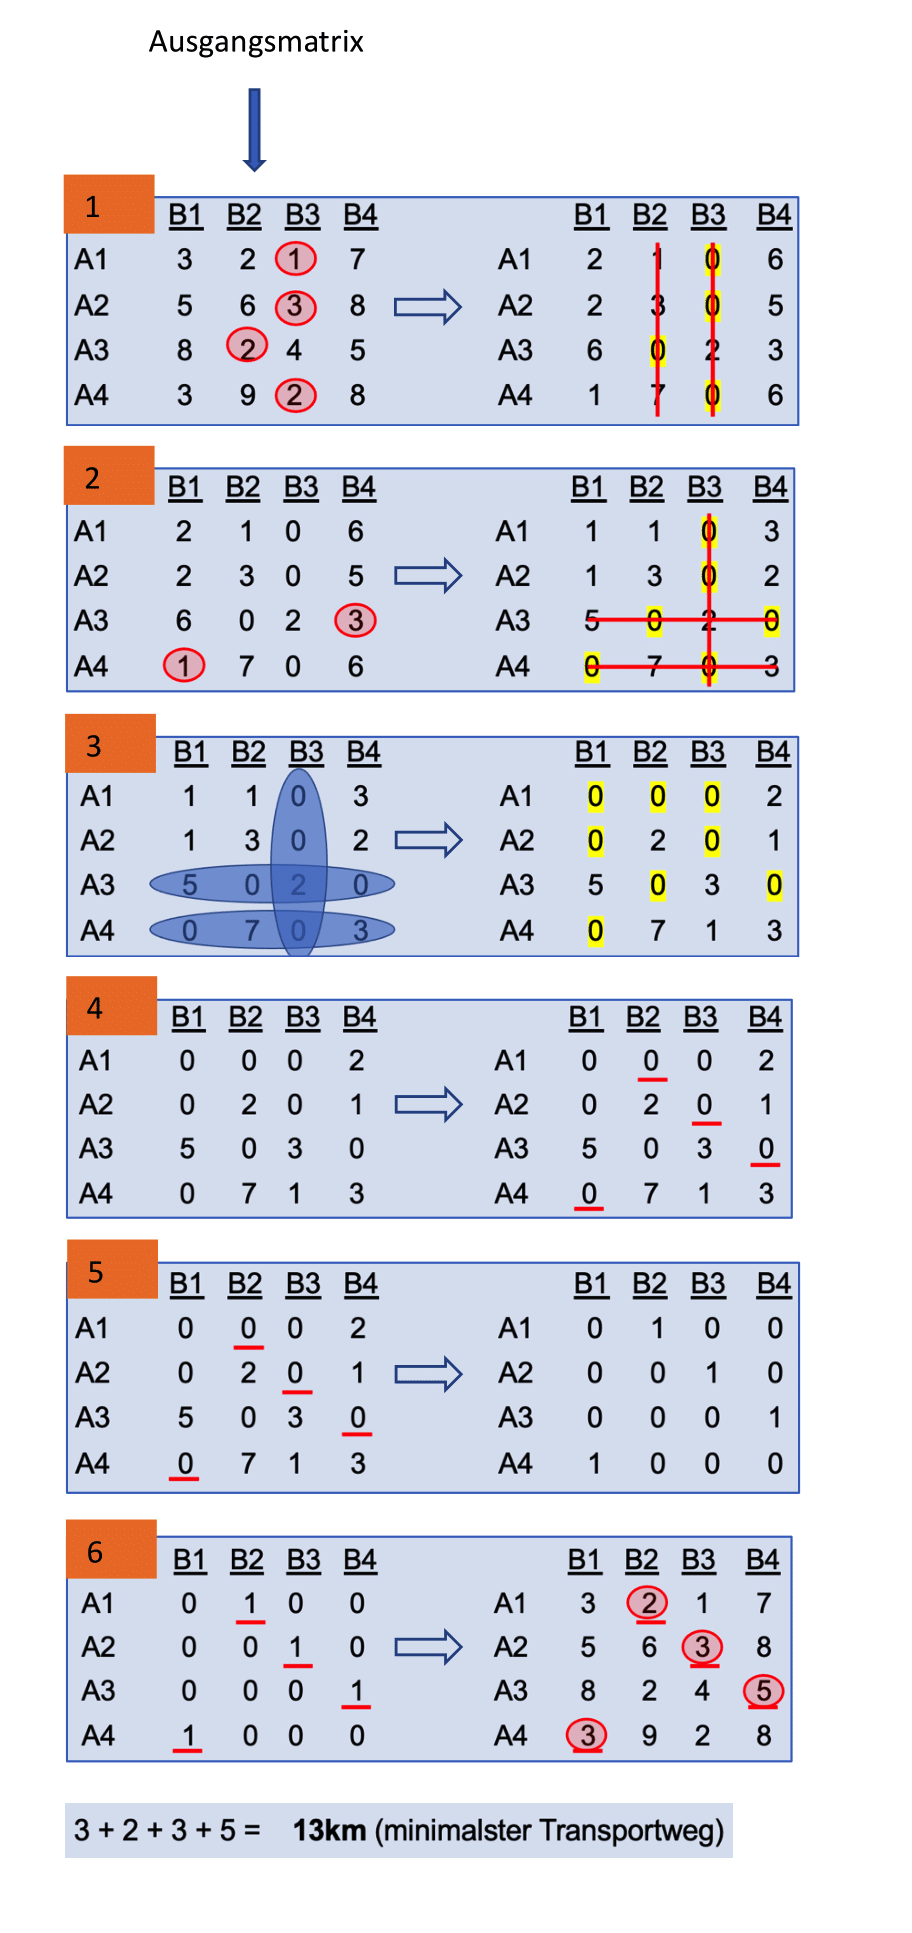
\includegraphics[width=14cm]{papers/munkres/figures/Ungarische_Methode_Beispiel.png}
\caption{Händisches Beispiel des Munkres Algorithmus, minimalster Transportweg.}
\label{munkres:Vr2}
\end{figure}

\subsection{Zuordnung der Kräne
\label{munkres:subsection:malorum}}

\begin{itemize}
\item Der Kran von Baustelle A1 soll zur Baustelle B2.
\item Der Kran von Baustelle A2 soll zur Baustelle B3.
\item Der Kran von Baustelle A3 soll zur Baustelle B4.
\item Der Kran von Baustelle A4 soll zur Baustelle B1.
\end{itemize}

\begin{figure}
\centering
\includegraphics[width=3cm]{papers/munkres/figures/Ungarische Methode Beispiel Zuweisung.png}
\caption{Händisches Beispiel des Munkres Algorithmus, Zuweisung der Kräne }
\label{munkres:Vr2}
\end{figure}

